\documentclass[aspectratio=1610,onlymath]{beamer}
% \documentclass[aspectratio=1610,onlymath,handout]{beamer}

\input{macros-lecture}
% Common notation

\usepackage{amsmath,amssymb,amsfonts}
\usepackage{xspace}

\newcommand{\lectureurl}{https://iccl.inf.tu-dresden.de/web/FS2023}

\DeclareMathAlphabet{\mathsc}{OT1}{cmr}{m}{sc} % Let's have \mathsc since the slide style has no working \textsc

% Dual of "phantom": make a text that is visible but intangible
\newcommand{\ghost}[1]{\raisebox{0pt}[0pt][0pt]{\makebox[0pt][l]{#1}}}

\newcommand{\tuple}[1]{\langle{#1}\rangle}
\newcommand{\defeq}{\mathrel{:=}}

%%% Annotation %%%

\usepackage{color}
\newcommand{\todo}[1]{{\tiny\color{red}\textbf{TODO: #1}}}



%%% Old macros below; move when needed

\newcommand{\blank}{\text{\textvisiblespace}} % empty tape cell for TM

% table syntax
\newcommand{\dom}{\textbf{dom}}
\newcommand{\adom}{\textbf{adom}}
\newcommand{\dbconst}[1]{\texttt{"#1"}}
\newcommand{\pred}[1]{\textsf{#1}}
\newcommand{\foquery}[2]{#2[#1]}
\newcommand{\ground}[1]{\textsf{ground}(#1)}
% \newcommand{\foquery}[2]{\{#1\mid #2\}} %% Notation as used in Alice Book
% \newcommand{\foquery}[2]{\tuple{#1\mid #2}}

\newcommand{\quantor}{\mathord{\reflectbox{$\text{\sf{Q}}$}}} % the generic quantor

% logic syntax
\newcommand{\Inter}{\mathcal{I}} %used to denote an interpretation
\newcommand{\Jnter}{\mathcal{J}} %used to denote another interpretation
\newcommand{\Knter}{\mathcal{K}} %used to denote yet another interpretation
\newcommand{\Zuweisung}{\mathcal{Z}} %used to denote a variable assignment

% query languages
\newcommand{\qlang}[1]{{\sf #1}} % Font for query languages
\newcommand{\qmaps}[1]{\textbf{QM}({\sf #1})} % Set of query mappings for a query language

%%% Complexities %%%

\hyphenation{Exp-Time} % prevent "Ex-PTime" (see, e.g. Tobies'01, Glimm'07 ;-)
\hyphenation{NExp-Time} % better that than something else

% \newcommand{\complclass}[1]{{\sc #1}\xspace} % font for complexity classes
\newcommand{\complclass}[1]{\ensuremath{\mathsc{#1}}\xspace} % font for complexity classes

\newcommand{\ACzero}{\complclass{AC$_0$}}
\newcommand{\LogSpace}{\complclass{L}}
\newcommand{\NLogSpace}{\complclass{NL}}
\newcommand{\PTime}{\complclass{P}}
\newcommand{\NP}{\complclass{NP}}
\newcommand{\coNP}{\complclass{coNP}}
\newcommand{\PH}{\complclass{PH}}
\newcommand{\PSpace}{\complclass{PSpace}}
\newcommand{\NPSpace}{\complclass{NPSpace}}
\newcommand{\ExpTime}{\complclass{ExpTime}}
\newcommand{\NExpTime}{\complclass{NExpTime}}
\newcommand{\ExpSpace}{\complclass{ExpSpace}}
\newcommand{\TwoExpTime}{\complclass{2ExpTime}}
\newcommand{\NTwoExpTime}{\complclass{N2ExpTime}}
\newcommand{\ThreeExpTime}{\complclass{3ExpTime}}
\newcommand{\kExpTime}[1]{\complclass{#1ExpTime}}
\newcommand{\kExpSpace}[1]{\complclass{#1ExpSpace}}


\usetikzlibrary{shapes}

\defineTitle{15}{Einleitung Kellerautomaten}{30. November 2023}

\begin{document}

\maketitle

\sectionSlideNoHandout{Rückblick}

\newcommand{\mytabnote}[2]{\ghost{#1}\hspace{2cm}{\textcolor{devilscss}{(#2)}}}
\newcommand{\myhitabnote}[2]{\ghost{#1}\hspace{2cm}{\textcolor{darkred}{#2}}}
\begin{frame}\frametitle{(Nicht)Abschlusseigenschaften für Typ 2}

\theobox{
\emph{Satz:} Wenn $\Slang{L}$, $\Slangsub{L}{1}$ und $\Slangsub{L}{2}$ kontextfreie Sprachen sind, dann beschreiben auch die
folgenden Ausdrücke kontextfreie \ghost{Sprachen:}%
\begin{enumerate}[(1)]%
\item \mytabnote{$\Slangsub{L}{1}\cup\Slangsub{L}{2}$}{Abschluss unter Vereinigung}
\item \mytabnote{$\Slangsub{L}{1}\circ\Slangsub{L}{2}$}{Abschluss unter Konkatenation}
\item \mytabnote{$\Slang{L}^*$}{Abschluss unter Kleene-Stern}
\end{enumerate}
}

Aber: 
\theobox{
\emph{Satz:} Es gibt kontextfreie Sprachen $\Slang{L}$, $\Slangsub{L}{1}$ und $\Slangsub{L}{2}$, so dass die folgenden
Ausdrücke keine kontextfreien Sprachen sind:
\begin{enumerate}[(1)]
\item \mytabnote{$\Slangsub{L}{1}\cap\Slangsub{L}{2}$}{Nichtabschluss unter Schnitt}
\item \mytabnote{$\overline{\Slang{L}}$}{Nichtabschluss unter Komplement}
\end{enumerate}
}

\end{frame}

\sectionSlide{Kellerautomaten}

\begin{frame}\frametitle{Ein Berechnungsmodell für Typ-2-Sprachen}

Eine typische Problemsprache (kontextfrei aber nicht regulär):
\medskip

\narrowcentering{{\huge$\{\Sterm{a}^i\Sterm{b}^i\mid i\geq 0\}$}}
\bigskip

Warum können endliche Automaten diese Sprache nicht erkennen?\pause

\begin{center}
\alert{{\large Weil sie die Zahl der gelesenen \Sterm{a}\\nicht \redalert{speichern} können.}}
\end{center}

$\leadsto$ Wir wollen endlichen Automaten mehr Speicher geben.

\end{frame}

\begin{frame}\frametitle{Pseudoalgorithmus $\{\Sterm{a}^i\Sterm{b}^i\mid i\geq 0\}$}

\begin{minipage}{5.2cm}
\codebox{
{\footnotesize\tt%
\Scode{function} isAiBi():\\
~~state = \Scodelit{"{}readA"{}}\\
~~anum  = \Scodelit{0}\\
~~\Scode{while} hasNextSymbol():\\
~~~~symbol = getNextSymbol()\\[1ex]
~~~~\Scode{if} ( state == \Scodelit{"{}readA"{}} ):\\
~~~~~~\Scode{if} ( symbol == \Sterm{a} ):\\
~~~~~~~~anum = anum + \Scodelit{1}\\
~~~~~~\Scode{else if} ( symbol == \Sterm{b} ):\\
~~~~~~~~anum = anum - \Scodelit{1}\\
~~~~~~~~state = \Scodelit{"{}readB"{}}\\[1ex]
~~~~\Scode{else if} ( state == \Scodelit{"{}readB"{}} ):\\
~~~~~~\Scode{if} ( symbol == \Sterm{a} ):\\
~~~~~~~~\Scode{return} \Scodelit{false}\\
~~~~~~\Scode{else if} ( symbol == \Sterm{b} ):\\
~~~~~~~~anum = anum - \Scodelit{1}\\[1ex]
~~\Scode{return} ( anum == \Scodelit{0} )
}}
\end{minipage}\hspace{8mm}\pause%
\begin{minipage}{3.9cm}
Speicherbedarf?\pause
\begin{itemize}
\item Zustandsvariable \texttt{state} (1bit -- zwei mögliche Werte)
\item Zähler \texttt{anum} (beliebig große Zahl!)
\end{itemize}

\begin{flushleft}
\alert{Der Algorithmus benötigt eine unbeschränkte Menge an Speicher, je nach Eingabe}\\
\end{flushleft}
$\leadsto$ kein endlicher Automat
\end{minipage}

\end{frame}

\begin{frame}\frametitle{Endliche Automaten + Speicher}

Das vorige Beispiel verwendet eine Zustandsvariable, fast wie ein endlicher Automat \ldots
\bigskip

\anybox{lime}{Wir müssten endliche Automaten irgendwie durch einen unbegrenzt großen "`Speicher"' ergänzen. Aber welche Form soll dieser Speicher haben?}%
\vspace{-5mm}

\narrowcentering{%
\begin{tikzpicture}[
	scale=0.50,
	decoration=penciline, decorate
]
% \path[use as bounding box] (-3.2,0) rectangle (3.5,-5); % add "draw" to see it
% \draw[help lines] (0,0) grid (5,5);
\pgfmathsetseed{5712}
%
\node (inlabel) [circle,draw=none,inner sep=1pt] at (2,0.5) {\alert{Eingabewort}};
\draw[fill=none,decorate,line width=0.3mm] (0,0) -- (6,0);
\draw[fill=none,decorate,line width=0.3mm] (0,-1) -- (6,-1);
\foreach \x in {0,...,4} {
	\draw[fill=none,decorate,line width=0.3mm] (\x,0) -- (\x,-0.9);
	\node (s\x) [circle,draw=none,inner sep=1pt] at (\x+0.5,-0.5) {\ifthenelse{\x<4}{\Sterm{a}}{\Sterm{b}}};
}
\draw[fill=none,decorate,line width=0.3mm] (5,0) -- (5,-0.9);
\node (dots) [circle,draw=none,inner sep=1pt] at (5.8,-0.5) {$\cdots$};

\draw[fill=none,decorate,line width=0.3mm]
	(2,-3) -- (6,-3) -- (6,-7) -- (2,-7) -- cycle;
\node (falabel) [circle,draw=none,inner sep=1pt,align=left] at (4,-5) {Endliche\\Steuerung};
\draw[fill=none,decorate,line width=0.4mm,darkblue,->]
	(4,-3) -- (4,-2) -- (1.5,-2) -> (1.5,-1);

\node[rectangle,align=center,draw,line width=0.3mm,decorate, minimum width=8mm, minimum height=8mm] (state) at (8, -6) {$q$};
\draw[fill=none,decorate,line width=0.4mm,darkblue,->]
	(6,-6) -> (state.180);
\node (qlabel) [circle,draw=none,inner sep=1pt] at (11.5,-6) {\footnotesize\alert{Zustandsvariable}};

\visible<2->{
\node[cloud, cloud puffs=15.7, cloud ignores aspect, minimum width=4cm, minimum height=1cm, align=center, draw,line width=0.3mm] (memory) at (11, -1) {\alert{zusätzlicher}\\\alert{Speicher}};
\draw[fill=none,decorate,line width=0.4mm,darkblue,->]
	(6,-4) -- (11.2,-4) -- (11.2,-2.9);
}
\end{tikzpicture}}

\end{frame}


\begin{frame}\frametitle{Welche Form hat der Speicher?}

Das vorige Beispiel verwendet eine beliebig große \alert{Zahl}.\pause
\medskip

Im Allgemeinen sind Zahlen aber nicht das sinnvollste Format für die Speicherung der
Informationen, die beim Erkennen kontextfreier Sprachen anfallen
\medskip

\examplebox{\emph{Beispiel:}
Die folgende kontextfreie Grammatik erkennt Palindrome über $\Sigma=\{\Sterm{a},\Sterm{b}\}$, deren Mitte mit $\Sterm{c}$ markiert ist:
\[ \Snterm{S} \to \Sterm{a} \Snterm{S} \Sterm{a} \mid \Sterm{b} \Snterm{S} \Sterm{b}\mid \Sterm{c}\]
Die Grammatik generiert zum Beispiel die Wörter \Sterm{abcba} und \Sterm{abaabcbaaba}.\medskip

Diese Sprache ist ebenfalls nicht regulär (Übung).
}

Wie würde man die Sprache aus diesem Beispiel erkennen?

\end{frame}

\begin{frame}\frametitle{Pseudoalgorithmus für markierte Palindrome}

\begin{minipage}{5.4cm}
\codebox{
{\footnotesize\tt%
\Scode{function} isMarkedPalindrome():\\
~~state = \Scodelit{"{}start"{}}\\
~~list = new Array()\\
~~\Scode{while} hasNextSymbol():\\
~~~~symbol = getNextSymbol()\\[0.5ex]
~~~~\Scode{if} ( state == \Scodelit{"{}start"{}} ):\\
~~~~~~\Scode{if} ( symbol == \Sterm{c} ):\\
~~~~~~~~state = \Scodelit{"{}end"{}}\\
~~~~~~\Scode{else}:\\
~~~~~~~~list.append(symbol)\\[0.5ex]
~~~~\Scode{else if} ( state == \Scodelit{"{}end"{}} ):\\
~~~~~~\Scode{if} ( !list.isEmpty() \&\&\\
~~~~~~~~symbol == \ghost{list.lastEntry() ):}\\
~~~~~~~~list.removeLastEntry()\\
~~~~~~\Scode{else}:\\
~~~~~~~~\Scode{return} \Scodelit{false}\\[0.5ex]
~~\Scode{return} ( list.isEmpty() )
}}
\end{minipage}\hspace{3mm}\pause%
\begin{minipage}{3.8cm}
~~~~Speicherformat?\pause
\begin{itemize}
\item Liste von Symbolen
\item Zugriffsmethoden:\\
{\footnotesize
\texttt{list.append(symbol)}\\
\texttt{list.lastEntry()}\\
\texttt{list.removeLastEntry()}\\
\texttt{list.isEmpty()}
}
\end{itemize}\pause

~~~~~\redalert{$\leadsto$ Stack (Keller)}

% \begin{flushleft}
% \alert{Der Algorithmus benötigt eine unbeschränkte Menge an Speicher, je nach Eingabe}\\
% \end{flushleft}
% $\leadsto$ kein endlicher Automat
\end{minipage}

\end{frame}

\begin{frame}\frametitle{Keller sind Stapel}

\anybox{gray}{
Ein \redalert{Stack} (oder auch \redalert{Keller} oder auch \redalert{Stapel}) ist eine 
Datenstruktur, die eine Liste von Einträgen speichert.\medskip

Wir denken uns die Liste vertikal, letzte Einträge oben\\(daher der Name).
\medskip

Wichtigste Zugriffsoperationen:
\begin{itemize}
\item \texttt{push}: ein Element wird oben auf dem Stapel abgelegt
\item \texttt{pop}: das oberste Element wird vom Stapel entfernt und zurückgegeben
(wenn der Stapel nicht leer ist)
\end{itemize}
Keller sind demnach \redalert{LIFO-Speicher} (last-in/first-out).

}\bigskip

\emph{Idee:} Verwende Keller als zusätzliche Speicher in endlichen Automaten

\end{frame}

\begin{frame}\frametitle{Automaten mit Kellern}

\alert{Wie kann ein Automat einen Keller lesen oder schreiben?}
\pause\bigskip

\begin{minipage}{4.2cm}\begin{flushleft}
\emph{Zustandsänderungen bei endlichen Automaten:}\\[1ex]
% 
Abhängig von\\
-- aktuellem Zustand\\
-- Eingabesymbol\\
~\\[1ex]
% 
Bestimme neuen Zustand\\
~\\[1ex]
%
\emph{Beispiel:} "`Wenn in Zustand $q_1$ Symbol \Sterm{a} gelesen wird, 
wechsle in Zustand $q_2$."'\\
~\\~
\end{flushleft}\end{minipage}\hspace{15mm}\pause%
\begin{minipage}{5.1cm}\begin{flushleft}
\emph{Zustandsänderungen bei endlichen Automaten mit Keller:}\\[1ex]
% 
Abhängig von\\
-- aktuellem Zustand\\
-- Eingabesymbol\\
-- oberstem Kellersymbol\\[1ex]
% 
Bestimme neuen Zustand\\
Schreibe auf Keller\\[1ex]
%
\emph{Beispiel:} "`Wenn in Zustand $q_1$ Symbol \Sterm{a} gelesen wird und Symbol $\Snterm{C}$
vom Keller gelesen wird, dann
wechsle in Zustand $q_2$ und schreibe $\Snterm{D}$ auf den Keller."'
\end{flushleft}\end{minipage}

\end{frame}

\begin{frame}\frametitle{Kellerautomaten definieren}

\alert{Übergangsfunktion von Kellerautomaten:}\\
~~\emph{Eingabe:} Zustand + Eingabesymbol + Kellersymbol (\texttt{pop})\\
~~\emph{Ausgabe:} Zustand + Kellersymbol (\texttt{push})
\bigskip\pause

\alert{Weitere Designentscheidungen:}
\begin{itemize}
\item Wir unterscheiden mögliche Eingabesymbole $\Sigma$ von\\möglichen Kellersymbolen $\Gamma$ (Gamma)\\
% \alert{$\leadsto$ Eingabealphabet $\Sigma$ + Kelleralphabet $\Gamma$ (Gamma)}
%
\pause
\item Wir wollen erlauben:
\begin{enumerate}[(1)]
\item dass der Automat manchmal kein Eingabesymbol liest\\
($\epsilon$-Übergänge)\pause
\item dass der Automat manchmal kein Kellersymbol liest
% \\\alert{$\leadsto$ wie $\epsilon$-Übergänge, aber bzgl. Kellersymbol}
\pause
\item dass der Automat manchmal nichts auf den Keller schreibt
% \\\alert{$\leadsto$ kodiert durch Schreiben von $\epsilon$ auf Keller}
\pause
\end{enumerate}
%
\item Wir wollen Kellerautomaten als nichtdeterministische Automaten definieren\\
$\leadsto$ Übergangsfunktion liefert Menge von Möglichkeiten
\end{itemize}

\end{frame}

\begin{frame}\frametitle{Kellerautomaten}

Zur Vereinfachung der folgenden Definition schreiben wir $\Sigma_\epsilon$ für $\Sigma\cup\{\epsilon\}$\\ (und analog für $\Gamma_\epsilon$).\bigskip

\defbox{Ein \redalert{Kellerautomat} (international: "`\alert{PDA}"'/"`\alert{Pushdown Automaton}"') 
\Smach{M} ist ein Tupel $\Smach{M}=\tuple{Q,\Sigma,\Gamma,\delta,Q_0,F}$ mit
den folgenden Bestandteilen:
\begin{itemize}
\item $Q$: endliche Menge von \redalert{Zuständen}
\item $\Sigma$: \redalert{Eingabealphabet}
\item $\Gamma$: \redalert{Kelleralphabet}
\item $\delta$: \redalert{Übergangsfunktion}, eine totale Funktion\\[1ex]
\narrowcentering{$Q\times\Sigma_\epsilon\times\Gamma_\epsilon \to 2^{Q\times\Gamma_\epsilon}$,}\\[1ex]
~~~~wobei $2^{Q\times\Gamma_\epsilon}$ die Potenzmenge von $Q\times\Gamma_\epsilon$ ist
\item $Q_0$: Menge möglicher \redalert{Startzustände} $Q_0\subseteq Q$
\item $F$: Menge von \redalert{Endzuständen} $F\subseteq Q$
\end{itemize}

}

\end{frame}

\begin{frame}[t]\frametitle{Kellerautomaten: Intuition (1)}

\defbox{
$\delta$: \redalert{Übergangsfunktion}, eine totale Funktion
$Q\times\Sigma_\epsilon\times\Gamma_\epsilon \to 2^{Q\times\Gamma_\epsilon}$.}\\[1ex]

\emph{Beispiele:}
\begin{itemize}
\item $\tuple{q_2,\Snterm{D}}\in\delta(q_1,\Sterm{a},\Snterm{C})$ bedeutet:\\
"`Wenn der PDA in Zustand $q_1$ das Symbol \Sterm{a} einliest und $\Snterm{C}$ oben vom Keller nimmt (\texttt{pop}),
dann \alert{kann} er in Zustand $q_2$ wechseln und dabei $\Snterm{D}$ auf den Keller legen (\texttt{push})."'\pause
%
\item $\tuple{q_2,\epsilon}\in\delta(q_1,\Sterm{a},\epsilon)$ bedeutet:\\
"`Wenn der PDA in Zustand $q_1$ das Symbol \Sterm{a} einliest, dann \alert{kann} er in Zustand $q_2$ wechseln (Keller bleibt unverändert)."'\pause
%
\item $\tuple{q_2,\Snterm{D}}\in\delta(q_1,\epsilon,\Snterm{C})$ bedeutet:\\
"`Wenn der PDA in Zustand $q_1$ das Symbol $\Snterm{C}$ oben vom Keller nimmt (\texttt{pop}),
dann \alert{kann} er in Zustand $q_2$ wechseln und dabei $\Snterm{D}$ auf den Keller legen (\texttt{push}),
ohne ein Symbol zu lesen."'
\end{itemize}
% \vspace{-3cm}~

\end{frame}

\begin{frame}[t]\frametitle{Kellerautomaten: Intuition (2)}

\defbox{
$\delta$: \redalert{Übergangsfunktion}, eine totale Funktion
$Q\times\Sigma_\epsilon\times\Gamma_\epsilon \to 2^{Q\times\Gamma_\epsilon}$.}\\[1ex]

\emph{Beispiele:}
\begin{itemize}
\item $\tuple{q_2,\Snterm{D}}\in\delta(q_1,\epsilon,\epsilon)$ bedeutet:\\
"`Wenn der PDA in Zustand $q_1$ ist, dann \alert{kann} er spontan in Zustand $q_2$ wechseln und dabei $\Snterm{D}$ auf den Keller legen (\texttt{push}), ohne dabei eine Eingabe oder den Keller zu lesen."'\pause
\item $\delta(q_1,\Sterm{a},\Snterm{C})=\emptyset$ bedeutet:\\
"`Wenn der PDA in Zustand $q_1$ das Symbol \Sterm{a} einliest und $\Snterm{C}$ oben vom Keller nimmt (\texttt{pop}),
dann kann er nichts mehr tun (kein erfolgreicher Lauf)."'
\item \ldots{} und viele andere Varianten
\end{itemize}

\end{frame}

\begin{frame}\frametitle{Beispiel $\{\Sterm{a}^i\Sterm{b}^i\mid i\geq 0\}$}

Ein PDA für $\{\Sterm{a}^i\Sterm{b}^i\mid i\geq 0\}$ könnte wie folgt aussehen:

\begin{itemize}
\item $\Sigma=\{\Sterm{a},\Sterm{b}\}$
\item $\Gamma=\{\Snterm{A},\Snterm{S}\}$
\item $Q=\{q_s,q_a,q_b,q_f\}$
\item $Q_0=\{q_s\}$
\item $F=\{q_s,q_f\}$
\end{itemize}

Wir definieren $\delta$ wie folgt:
\begin{itemize}
\item $\delta(q_s,\epsilon,\epsilon)=\{\tuple{q_a,\Snterm{S}}\}$ (markiere Kellerboden)
\item $\delta(q_a,\Sterm{a},\epsilon)=\{\tuple{q_a,\Snterm{A}}\}$ (speichere \Sterm{a})
\item $\delta(q_a,\Sterm{b},\Snterm{A})=\{\tuple{q_b,\epsilon}\}$ (erstes \Sterm{b})
\item $\delta(q_b,\Sterm{b},\Snterm{A})=\{\tuple{q_b,\epsilon}\}$ (weitere \Sterm{b})
\item $\delta(q_b,\epsilon,\Snterm{S})=\{\tuple{q_f,\epsilon}\}$ (mögliches Wortende)
\end{itemize}
Dies sind alle Übergänge (alle anderen Fälle liefern $\emptyset$)

\end{frame}

\begin{frame}\frametitle{Grafische Darstellung von PDAs}

\anybox{lime}{
Wir können PDAs ähnlich zu NFAs darstellen, wenn wir die Änderungen des Kellerinhalts
zusätzlich an die Übergänge schreiben.}\medskip

Beispiel des vorigen PDA für $\{\Sterm{a}^i\Sterm{b}^i\mid i\geq 0\}$:
\bigskip

\narrowcentering{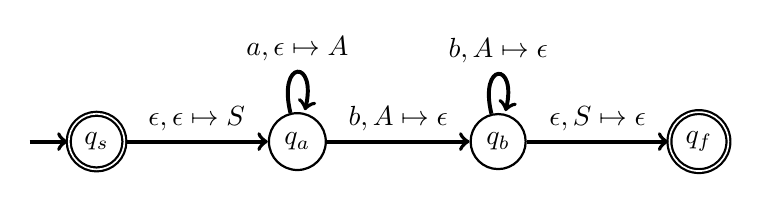
\begin{tikzpicture}[xscale=0.85,baseline={([yshift=-2ex]current bounding box.north)}]
% \draw[help lines] (0,0) grid (7,2);
\node (s) [circle,draw=black,thick,double] at (0,0) {$q_s$};
\node (a) [circle,draw=black,thick] at (3,0) {$q_a$};
\node (b) [circle,draw=black,thick] at (6,0) {$q_b$};
\node (f) [circle,draw=black,thick,double] at (9,0) {$q_f$};
%
\path[->,line width=0.5mm](-1,0) edge (s);
\path[->,line width=0.5mm](s) edge node[above] {$\epsilon,\epsilon\mapsto\Snterm{S}$} (a);
\path[->,line width=0.5mm](a) edge [loop above] node[above] {$\Sterm{a},\epsilon\mapsto\Snterm{A}$} (a);
\path[->,line width=0.5mm](a) edge node[above] {$\Sterm{b},\Snterm{A}\mapsto\epsilon$} (b);
\path[->,line width=0.5mm](b) edge [loop above] node[above] {$\Sterm{b},\Snterm{A}\mapsto\epsilon$} (b);
\path[->,line width=0.5mm](b) edge node[above] {$\epsilon,\Snterm{S}\mapsto\epsilon$} (f);
\end{tikzpicture}}\bigskip

\alert{Kodierungstrick:} Wir implementieren hier die Funktion \texttt{isEmpty} indem wir den Kelleranfang mit
einem speziellen Symbol $\Snterm{S}$ markieren, welches den (fast) leeren Keller signalisiert.

\end{frame}

\begin{frame}\frametitle{Beispiel: Palindrome ohne Markierung}

Wir betrachten die Sprache aller Palindrome über $\{\Sterm{a},\Sterm{b}\}$ mit gerader Wortlänge,
d.h. die Sprache $\{w w^r\mid w\in\{\Sterm{a},\Sterm{b}\}^*\}$ wobei $w^r$ die rückwärts gelesene Version von $w$ ist.
\pause

\bigskip
Wir können diese mit folgendem PDA
erkennen ($\Gamma=\{\Snterm{A},\Snterm{B},\Snterm{S}\}$):\bigskip

\narrowcentering{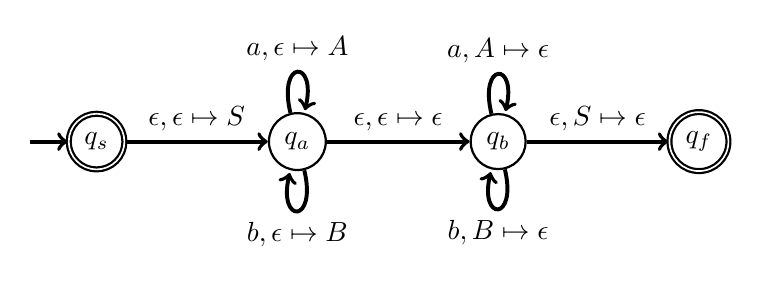
\begin{tikzpicture}[xscale=0.85,baseline={([yshift=-2ex]current bounding box.north)}]
% \draw[help lines] (0,0) grid (7,2);
\node (s) [circle,draw=black,thick,double] at (0,0) {$q_s$};
\node (a) [circle,draw=black,thick] at (3,0) {$q_a$};
\node (b) [circle,draw=black,thick] at (6,0) {$q_b$};
\node (f) [circle,draw=black,thick,double] at (9,0) {$q_f$};
%
\path[->,line width=0.5mm](-1,0) edge (s);
\path[->,line width=0.5mm](s) edge node[above] {$\epsilon,\epsilon\mapsto\Snterm{S}$} (a);
\path[->,line width=0.5mm](a) edge [loop above] node[above] {$\Sterm{a},\epsilon\mapsto\Snterm{A}$} (a);
\path[->,line width=0.5mm](a) edge [loop below] node[below] {$\Sterm{b},\epsilon\mapsto\Snterm{B}$} (a);
%
% \path[->,line width=0.5mm,bend left=20](a) edge node[above] {$\Sterm{a},\Snterm{A}\mapsto\epsilon$} (b);
% \path[->,line width=0.5mm,bend right=20](a) edge node[below] {$\Sterm{b},\Snterm{B}\mapsto\epsilon$} (b);
\path[->,line width=0.5mm](a) edge node[above] {$\epsilon,\epsilon\mapsto\epsilon$} (b);
\path[->,line width=0.5mm](b) edge [loop above] node[above] {$\Sterm{a},\Snterm{A}\mapsto\epsilon$} (b);
\path[->,line width=0.5mm](b) edge [loop below] node[below] {$\Sterm{b},\Snterm{B}\mapsto\epsilon$} (b);
\path[->,line width=0.5mm](b) edge node[above] {$\epsilon,\Snterm{S}\mapsto\epsilon$} (f);
\end{tikzpicture}}\bigskip

\alert{Anmerkung:} Wir erraten hier die Wortmitte nichtdeterministisch.

\end{frame}

\begin{frame}\frametitle{Konfigurationen eines PDA}

Wir können die Architektur von PDAs wie folgt veranschaulichen:

\narrowcentering{%
\begin{tikzpicture}[
	scale=0.50,
	decoration=penciline, decorate
]
% \path[use as bounding box] (-3.2,0) rectangle (3.5,-5); % add "draw" to see it
% \draw[help lines] (0,0) grid (5,5);
\pgfmathsetseed{5712}
%
\node (inlabel) [circle,draw=none,inner sep=1pt] at (2,0.5) {\alert{Eingabewort}};
\draw[fill=none,decorate,line width=0.3mm] (0,0) -- (6,0);
\draw[fill=none,decorate,line width=0.3mm] (0,-1) -- (6,-1);
\foreach \x in {0,...,4} {
	\draw[fill=none,decorate,line width=0.3mm] (\x,0) -- (\x,-0.9);
	\node (s\x) [circle,draw=none,inner sep=1pt] at (\x+0.5,-0.5) {\ifthenelse{\x<4}{\Sterm{a}}{\Sterm{b}}};
}
\draw[fill=none,decorate,line width=0.3mm] (5,0) -- (5,-0.9);
\node (dots) [circle,draw=none,inner sep=1pt] at (5.8,-0.5) {$\cdots$};

\draw[fill=none,decorate,line width=0.3mm]
	(2,-3) -- (6,-3) -- (6,-7) -- (2,-7) -- cycle;
\node (falabel) [circle,draw=none,inner sep=1pt,align=left] at (4,-5) {Endliche\\Steuerung};
\draw[fill=none,decorate,line width=0.4mm,darkblue,->]
	(4,-3) -- (4,-2) -- (1.5,-2) -> (1.5,-1);

\node[rectangle,align=center,draw,line width=0.3mm,decorate, minimum width=8mm, minimum height=8mm] (state) at (8, -6) {$q$};
\draw[fill=none,decorate,line width=0.4mm,darkblue,->]
	(6,-6) -> (state.180);
\node (qlabel) [circle,draw=none,inner sep=1pt] at (11.5,-6) {\footnotesize\alert{Zustandsvariable}};

% \node[cloud, cloud puffs=15.7, cloud ignores aspect, minimum width=4cm, minimum height=1cm, align=center, draw,line width=0.3mm] (memory) at (11, -1) {\alert{zusätzlicher}\\\alert{Speicher}};

\draw[fill=none,decorate,line width=0.3mm] (9,0) -- (9,-4);
\draw[fill=none,decorate,line width=0.3mm] (10,0) -- (10,-4);
\draw[fill=none,decorate,line width=0.3mm] (8.5,-4) -- (10.5,-4);
\foreach \y in {0,...,-3} {
	\draw[fill=none,decorate,line width=0.3mm] (9,\y) -- (10,\y);
	\node (k\y) [circle,draw=none,inner sep=1pt] at (9.5,\y-0.5) {\ifthenelse{\y<-1}{\Snterm{A}}{\Snterm{B}}};
}
\draw[fill=none,decorate,line width=0.4mm,darkblue,->]
	(6,-3.5) -- (7.5,-3.5) -- (7.5,-0.5) -> (9,-0.5);
\node (stacklabel) [circle,draw=none,inner sep=1pt] at (11.5,-2.5) {\alert{Keller}};
\end{tikzpicture}}

Eine mögliche \redalert{Konfiguration} des PDA während der Erkennung ist gegeben durch
den Zustand $q\in Q$, den Inhalt des Kellers $\gamma\in\Gamma^*$ und das noch zu lesende Restwort $w\in\Sigma^*$.

% Wir können auch für PDAs eine Übergangsfunktion definieren:

\end{frame}

\begin{frame}\frametitle{Die Sprache eines PDA (formal)}

Sei $\Smach{M}=\tuple{Q,\Sigma,\Gamma,\delta,Q_0,F}$ ein PDA.

\defbox{Eine \redalert{Konfiguration} von $\Smach{M}$ ist ein Tripel
$\tuple{q,w,\gamma}\in Q\times \Sigma^*\times \Gamma^*$.
Wir definieren eine \redalert{Übergangsrelation} zwischen Konfigurationen wie folgt.\medskip

Die Konfiguration $\tuple{q,vw,\psi\gamma}$ kann in die Konfiguration $\tuple{q',w,\psi'\gamma}$ übergehen,
in Symbolen $\tuple{q,vw,\psi\gamma}\vdash\tuple{q',w,\psi'\gamma}$, 
falls gilt $\tuple{q',\psi'}\in \delta(q,v,\psi)$.\footnote{\textcolor{devilscss}{Anmerkung: In diesem Fall ist $v\in\Sigma_\epsilon$ und $\psi,\psi'\in\Gamma_\epsilon$.}}
Mit $\vdash^*$ bezeichnen wir den reflexiven, transitiven Abschluss von $\vdash$.
}

Dies entspricht der intuitiven Idee von möglichen Übergängen.

\defbox{Der PDA $\Smach{M}$ akzeptiert ein Wort $w$ wenn es Übergänge $\tuple{q_s,w,\epsilon}\vdash^* \tuple{q_f,\epsilon,\gamma}$ gibt für ein $q_s\in Q_0$ und $q_f\in F$. Die von $\Smach{M}$ akzeptierte Sprache $\Slang{L}(\Smach{M})$ ist die Menge aller von $\Smach{M}$ akzeptierten Wörter.
}

\end{frame}

\begin{frame}\frametitle{Beispiel}

Der Automat

\scalebox{1.0}{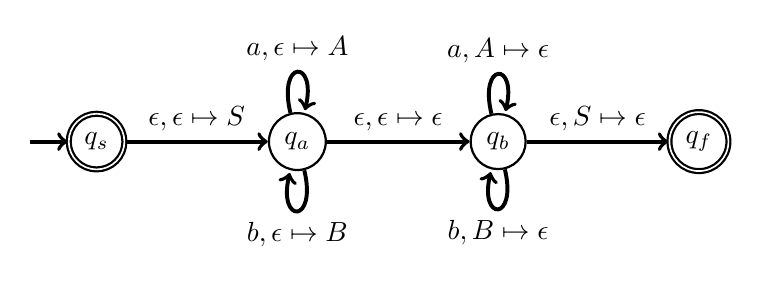
\begin{tikzpicture}[xscale=0.85,baseline={([yshift=-2ex]current bounding box.north)}]
% \draw[help lines] (0,0) grid (7,2);
\node (s) [circle,draw=black,thick,double] at (0,0) {$q_s$};
\node (a) [circle,draw=black,thick] at (3,0) {$q_a$};
\node (b) [circle,draw=black,thick] at (6,0) {$q_b$};
\node (f) [circle,draw=black,thick,double] at (9,0) {$q_f$};
%
\path[->,line width=0.5mm](-1,0) edge (s);
\path[->,line width=0.5mm](s) edge node[above] {$\epsilon,\epsilon\mapsto\Snterm{S}$} (a);
\path[->,line width=0.5mm](a) edge [loop above] node[above] {$\Sterm{a},\epsilon\mapsto\Snterm{A}$} (a);
\path[->,line width=0.5mm](a) edge [loop below] node[below] {$\Sterm{b},\epsilon\mapsto\Snterm{B}$} (a);
%
% \path[->,line width=0.5mm,bend left=20](a) edge node[above] {$\Sterm{a},\Snterm{A}\mapsto\epsilon$} (b);
% \path[->,line width=0.5mm,bend right=20](a) edge node[below] {$\Sterm{b},\Snterm{B}\mapsto\epsilon$} (b);
\path[->,line width=0.5mm](a) edge node[above] {$\epsilon,\epsilon\mapsto\epsilon$} (b);
\path[->,line width=0.5mm](b) edge [loop above] node[above] {$\Sterm{a},\Snterm{A}\mapsto\epsilon$} (b);
\path[->,line width=0.5mm](b) edge [loop below] node[below] {$\Sterm{b},\Snterm{B}\mapsto\epsilon$} (b);
\path[->,line width=0.5mm](b) edge node[above] {$\epsilon,\Snterm{S}\mapsto\epsilon$} (f);
\end{tikzpicture}}

erlaubt z.B. die folgenden Konfigurationsübergänge:
\bigskip

$\tuple{q_s,\Sterm{abba},\epsilon}
\vdash\tuple{q_a,\Sterm{abba},\Snterm{S}}
\vdash\tuple{q_a,\Sterm{bba},\Snterm{AS}}
\vdash\tuple{q_a,\Sterm{ba},\Snterm{BAS}}
\vdash\tuple{q_a,\Sterm{a},\Snterm{BBAS}}
\vdash\tuple{q_a,\epsilon,\Snterm{ABBAS}}$
(kein akzeptierender Lauf)\pause
\bigskip

$\tuple{q_s,\Sterm{abba},\epsilon}
\vdash\tuple{q_a,\Sterm{abba},\Snterm{S}}
\vdash\tuple{q_a,\Sterm{bba},\Snterm{AS}}
\vdash\tuple{q_a,\Sterm{ba},\Snterm{BAS}}
\vdash\tuple{q_b,\Sterm{ba},\Snterm{BAS}}
\vdash\tuple{q_b,\Sterm{a},\Snterm{AS}}
\vdash\tuple{q_b,\epsilon,\Snterm{S}}\vdash\tuple{q_f,\epsilon,\epsilon}$\\ (akzeptierender Lauf)
% \bigskip


\end{frame}

\begin{frame}\frametitle{PDA: Variationen}

Es gibt auch hier viele äquivalente Definitionen\pause
\begin{itemize}
\item Ein Startzustand reicht auch aus (Übung: warum?)\pause
\item Alternative Akzeptanzbedingung: ersetze "`PDA ist in Endzustand"' durch "`PDA hat leeren Keller"'
(keine Endzustände nötig, dafür manchmal aufwendigere Kodierung)\pause
% 
% Statt Endzustände zu verwenden kann man Terminierung von PDAs auch bei leerem Keller erlauben
\item Die Übergangsfunktion $\delta$ kann auch als Relation $\Delta\subseteq (Q\times\Sigma_\epsilon\times\Gamma_\epsilon)\times (Q\times\Gamma_\epsilon)$ beschrieben werden (wie bei \ghost{NFAs)}\pause
\item Das Startsymbol des Kellers kann Teil der Definition sein\pause
\item Man kann erlauben, dass in einem Schritt mehrere Symbole auf den Keller geschrieben werden.
\\ {\footnotesize \textcolor{devilscss}{Dann kann man auch verlangen, dass in jedem Schritt ein Symbol entnommen wird (\texttt{pop}), da man es bei Bedarf zurücklegen kann}}
\end{itemize}
\alert{Jede dieser Varianten führt zur gleichen Ausdrucksstärke}

\end{frame}

\begin{frame}\frametitle{Wörter \texttt{push}en}

Wir können Übergänge der folgenden Form erlauben:\medskip

\narrowcentering{%
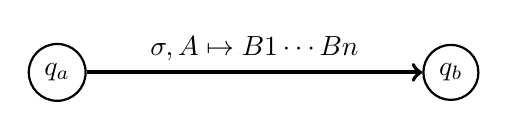
\begin{tikzpicture}[baseline={([yshift=-2ex]current bounding box.north)}]
% \draw[help lines] (0,0) grid (7,2);
\node (a) [circle,draw=black,thick] at (0,0) {$q_a$};
\node (b) [circle,draw=black,thick] at (5,0) {$q_b$};
%
\path[->,line width=0.5mm](a) edge node[above] {$\sigma,\Snterm{A}\mapsto\Sntermsub{B}{1}\cdots\Sntermsub{B}{n}$} (b);
\end{tikzpicture}}
\medskip

"`Wenn in Zustand $q_a$ das Zeichen (oder leere Wort) $\sigma$ gelesen wird\\
und wenn $\Snterm{A}$ oben vom Keller geholt werden kann (\texttt{pop}),\\
dann wechsle in Zustand $q_b$\\
und lege die Zeichen $\Sntermsub{B}{1}\cdots\Sntermsub{B}{n}$ auf den Keller\\
(wobei $\Sntermsub{B}{1}$ ganz oben zu liegen kommt)."'
\medskip\pause

Dies kann mithilfe neuer Zustände kodiert werden:\bigskip

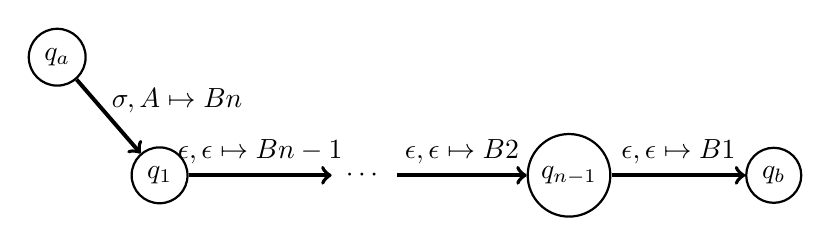
\begin{tikzpicture}[xscale=1.3,baseline={([yshift=-2ex]current bounding box.north)}]
% \draw[help lines] (0,0) grid (7,2);
\node (a) [circle,draw=black,thick] at (1,1.5) {$q_a$};
\node (n1) [circle,draw=black,thick] at (2,0) {$q_1$};
\node (n2) [circle,draw=none,thick] at (4,0) {$\cdots$};
\node (nm1) [circle,draw=black,thick] at (6,0) {$q_{n-1}$};
\node (b) [circle,draw=black,thick] at (8,0) {$q_b$};
%
\path[->,line width=0.5mm](a) edge node[right,yshift=2mm,xshift=-1mm] {$\sigma,\Snterm{A}\mapsto\Sntermsub{B}{n}$} (n1);
\path[->,line width=0.5mm](n1) edge node[above] {$\epsilon,\epsilon\mapsto\Sntermsub{B}{n-1}$} (n2);
\path[->,line width=0.5mm](n2) edge node[above] {$\epsilon,\epsilon\mapsto\Sntermsub{B}{2}$} (nm1);
\path[->,line width=0.5mm](nm1) edge node[above] {$\epsilon,\epsilon\mapsto\Sntermsub{B}{1}$} (b);
\end{tikzpicture}

\end{frame}



\begin{frame}\frametitle{Ausdrucksstärke von PDAs}

Man kann nun formal untersuchen, welche Sprachen durch PDAs akzeptiert werden können.
Wir erhalten das erhoffte Resultat:\medskip

\theobox{\emph{Satz:} Eine Sprache ist genau dann kontextfrei wenn sie von einem PDA akzeptiert wird.}\pause\bigskip
% \theobox{Satz: Eine Sprache $\Slang{L}$ ist kontextfrei genau dann wenn es einen PDA $\Smach{M}$ mit 
% $\Slang{L}(\Smach{M})=\Slang{L}$ gibt.}\pause\bigskip

Der Beweis erfolgt in zwei Schritten:
\begin{enumerate}[(1)]
\item Umwandlung Typ-2-Grammatik $\leadsto$ PDA
\item Umwandlung PDA $\leadsto$ Typ-2-Grammatik
\end{enumerate}

\end{frame}

\begin{frame}[t]\frametitle{Grammatik $\leadsto$ PDA}

Wir wollen zunächst eine Richtung zeigen:

\theobox{\emph{Satz:} Für jede kontextfreie Grammatik $G$ gibt es einen PDA $\Smach{P}_G$, so dass \ghost{$\Slang{L}(G)=\Slang{L}(\Smach{P}_G)$.}}\pause\bigskip

\emph{Beweisidee:}
\begin{itemize}
\item Der PDA simuliert eine Ableitung in der Grammatik
\item Der Keller speichert das Zwischenergebnis der Ableitung (Terminale und Nichtterminale), linke Zeichen zuoberst
\item Der PDA arbeitet das Zwischenergebnis von links ab:
\begin{itemize}
\item Terminale werden mit Eingabe verglichen und entfernt
\item Nichtterminale werden durch Grammatikregel ersetzt
\end{itemize}
\item Die Ableitung gelingt, wenn die gesamte Eingabe gelesen werden konnte und der Keller leer ist
\end{itemize}

\end{frame}

\begin{frame}[t]\frametitle{Grammatik $\leadsto$ PDA}

Wir wollen zunächst eine Richtung zeigen:

\theobox{\emph{Satz:} Für jede kontextfreie Grammatik $G$ gibt es einen PDA $\Smach{P}_G$, so dass \ghost{$\Slang{L}(G)=\Slang{L}(\Smach{P}_G)$.}}\bigskip

\emph{Beweis:} Sei $G=\tuple{V,\Sigma,P,\Snterm{S}}$.
Wir definieren einen erweiterten PDA\pause:\bigskip

\narrowcentering{%
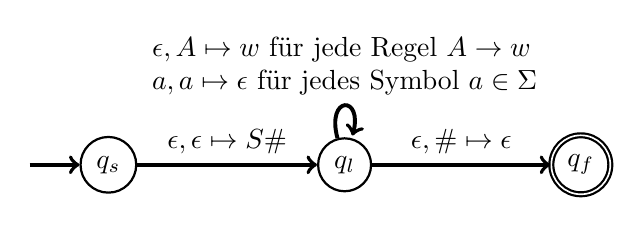
\begin{tikzpicture}[baseline={([yshift=-2ex]current bounding box.north)}]
% \draw[help lines] (0,0) grid (7,2);
\node (a) [circle,draw=black,thick] at (0,0) {$q_s$};
\node (b) [circle,draw=black,thick] at (3,0) {$q_l$};
\node (c) [circle,draw=black,thick,double] at (6,0) {$q_f$};
%
\path[->,line width=0.5mm](-1,0) edge (a);
\path[->,line width=0.5mm](a) edge node[above] {$\epsilon,\epsilon\mapsto\Snterm{S}\Snterm{\#}$} (b);
\path[->,line width=0.5mm](b) edge [loop above] node[above,align=left] {$\epsilon,\Snterm{A}\mapsto w$ für jede Regel $\Snterm{A}\to w$\\$\Sterm{a},\Sterm{a}\mapsto \epsilon$ für jedes Symbol $\Sterm{a}\in\Sigma$} (b);
\path[->,line width=0.5mm](b) edge node[above] {$\epsilon,\Snterm{\#}\mapsto\epsilon$} (c);
\end{tikzpicture}}\medskip\pause

Wir verwenden dabei also:\\[1ex]
\narrowcentering{$Q=\{q_s, q_l, q_f\}$\hfill $Q_0=\{q_s\}$\hfill $F=\{q_f\}$\hfill  $\Gamma=\Sigma\cup V\cup\{\Snterm{\#}\}$}\\[1ex]

Durch Entfernen der Wort-\texttt{push}-Operationen wie zuvor gezeigt entsteht der gesuchte PDA $\Smach{P}_G$.
\qed

\end{frame}

\begin{frame}\frametitle{Beispiel}

Die Grammatik $\Snterm{S}\to\Sterm{a}\Snterm{S}\Sterm{a}\mid\Sterm{b}\Snterm{S}\Sterm{b}\mid\epsilon$
ergibt den folgenden PDA:
\bigskip

\narrowcentering{%
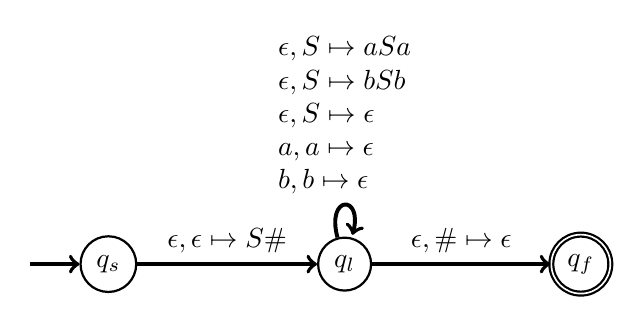
\begin{tikzpicture}[baseline={([yshift=-2ex]current bounding box.north)}]
% \draw[help lines] (0,0) grid (7,2);
\node (a) [circle,draw=black,thick] at (0,0) {$q_s$};
\node (b) [circle,draw=black,thick] at (3,0) {$q_l$};
\node (c) [circle,draw=black,thick,double] at (6,0) {$q_f$};
%
\path[->,line width=0.5mm](-1,0) edge (a);
\path[->,line width=0.5mm](a) edge node[above] {$\epsilon,\epsilon\mapsto\Snterm{S}\Snterm{\#}$} (b);
\path[->,line width=0.5mm](b) edge [loop above] node[above,align=left] {$\epsilon,\Snterm{S}\mapsto \Sterm{a}\Snterm{S}\Sterm{a}$\\$\epsilon,\Snterm{S}\mapsto \Sterm{b}\Snterm{S}\Sterm{b}$\\
$\epsilon,\Snterm{S}\mapsto \epsilon$\\
$\Sterm{a},\Sterm{a}\mapsto \epsilon$\\$\Sterm{b},\Sterm{b}\mapsto \epsilon$} (b);
\path[->,line width=0.5mm](b) edge node[above] {$\epsilon,\Snterm{\#}\mapsto\epsilon$} (c);
\end{tikzpicture}}\pause\bigskip

Mögliche Konfigurationsfolge (Wörter werden zur Vereinfachung in einem Schritt auf Stack geschrieben):
\medskip

$\tuple{q_s,\Sterm{abba},\epsilon}\pause
\vdash\tuple{q_l,\Sterm{abba},\Snterm{S}\Snterm{\#}}\pause
\vdash\tuple{q_l,\Sterm{abba},\Sterm{a}\Snterm{S}\Sterm{a}\Snterm{\#}}\pause
\vdash\tuple{q_l,\Sterm{bba},\Snterm{S}\Sterm{a}\Snterm{\#}}\pause
\vdash\tuple{q_l,\Sterm{bba},\Sterm{b}\Snterm{S}\Sterm{b}\Sterm{a}\Snterm{\#}}\pause
\vdash\tuple{q_l,\Sterm{ba},\Snterm{S}\Sterm{b}\Sterm{a}\Snterm{\#}}\pause
\vdash\tuple{q_l,\Sterm{ba},\Sterm{b}\Sterm{a}\Snterm{\#}}\pause
\vdash\tuple{q_l,\Sterm{a},\Sterm{a}\Snterm{\#}}\pause
\vdash\tuple{q_l,\epsilon,\Snterm{\#}}\pause
\vdash\tuple{q_f,\epsilon,\epsilon}$\\
~\hfill (akzeptierender Lauf)
\end{frame}


\begin{frame}\frametitle{Zusammenfassung und Ausblick}

\redalert{Kellerautomaten} (PDAs) erweitern endliche Automaten um einen unbeschränkt großen Speicher,
der aber nur nach dem LIFO-Prinzip verwendet werden kann.
\bigskip

PDAs erkennen genau die kontextfreien Sprachen.
\bigskip

Kontextfreie Grammatiken können durch sehr einfache PDAs (nichtdeterministisch) implementiert werden.\bigskip

\anybox{yellow}{
Offene Fragen:
\begin{itemize}
\item Wie geht der Beweis weiter?
\item Wie ist es mit deterministischen Kellerautomaten?
\item Welche Probleme auf kontextfreien Grammatiken kann man lösen?
\item Was gibt es zu Typ 1 und Typ 0 zu sagen?
\end{itemize}
}

\end{frame}


\end{document}
